% !TEX encoding = IsoLatin9

%%%%%%%%%%%%%%%%%%%%% SECTION 1
\section{Le perceptron}
\begin{frame}
  \begin{columns}
    \column{4.8cm}
    \tableofcontents[currentsection,hideothersubsections]
    \column{7cm}
      \centering{
      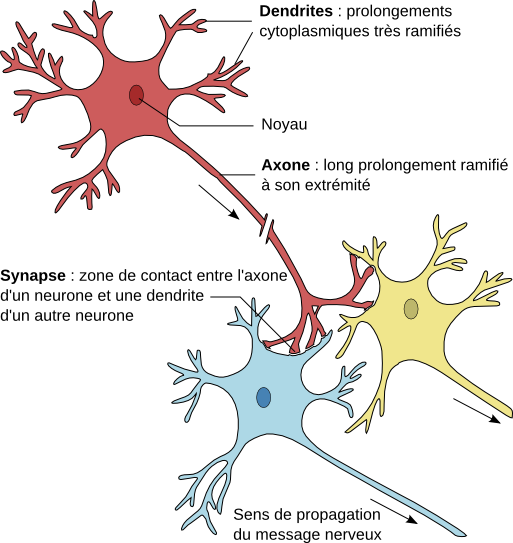
\includegraphics[width=6cm]{fig/neurone.png}
    }
  \end{columns}
  
\end{frame}


\begin{frame}
  \frametitle{Le perceptron : un neurone articiel}
  \begin{tikzpicture}[
    basic/.style={draw,fill=blue!20,text width=1em,text badly centered},
    input/.style={basic,circle},
    weights/.style={basic,rectangle},
functions/.style={basic,circle,fill=blue!10},
]
        \node[functions] (center) {};
        \node[below of=center,font=\scriptsize,text width=4em] {Fonction d'activation};
        \draw[thick] (0.5em,0.5em) -- (0,0.5em) -- (0,-0.5em) -- (-0.5em,-0.5em);
      %  \draw (0em,0.75em) -- (0em,-0.75em);
      %  \draw (0.75em,0em) -- (-0.75em,0em);
        \node[right of=center, anchor = west] (right) {$y=$ 0 ou 1};
            \path[draw,->] (center) -- (right);
        \node[functions,left=3em of center] (left) {$\sum$};
            \path[draw,->] (left) -- (center);
%        \node[weights,left=3em of left] (2) {$w_2$} -- (2) 
            \node[input,left= 4em of left] (l2) {$x_2$};
%            \path[draw,->] (l2) -- (2);
            \path[draw,->] (l2) -- node[above,midway]{$w_2$}(left);
        \node[below of=l2] (dots) {$\vdots$} ;
%(dots) node[left of=dots] (ldots) {$\vdots$};
%        \node[weights,below of=dots] (n) {$w_n$} -- (n) 
\node[input,below of=dots] (ln) {$x_n$};
%            \path[draw,->] (ln) -- (n);
            \path[draw,->] (ln) -- node[above,midway]{$w_n$}(left);
%        \node[weights,above of=2] (1) {$w_1$} -- (1) 
            \node[input,above of=l2] (l1) {$x_1$};
%            \path[draw,->] (l1) -- (1);
            \path[draw,->] (l1) -- node[above,midway]{$w_1$}(left);
%        \node[weights,above of=1] (0) {$w_0$} -- (0) 
\node[input,above of=l1] (l0) {$1$};
%            \path[draw,->] (l0) -- (0);
            \path[draw,->] (l0) -- node[above,midway]{$w_0$}(left);
        \node[below of=ln,font=\scriptsize](lin) {inputs};
        \node[right of=lin,font=\scriptsize] {weights};
    \end{tikzpicture}
\begin{block}{}
Si $w_0 + w_1\times x_1 + w_2\times x_2 +  \dots + w_n\times x_n < 0$, $\mathbf{y=0}$\\
sinon $\mathbf{y=1}$
\end{block}

\end{frame}

\begin{frame}[fragile]
\frametitle{En C, une structure de donn�es}
\begin{codeblock}{}
\vspace{-.3cm}
\lstset{escapeinside={��}}
%\lstset{basicstyle=\scriptsize}
\begin{codeC}
struct perceptron {
  short X[N] ; //entr�es
  short Y ; //sorties
  int W[N+1] ; //poids
  } ;
  
void active (struct perceptron *p) ;
\end{codeC}
\vspace{-.3cm}
\end{codeblock}
\end{frame}

\begin{frame}
\frametitle{Qu'est-ce que l'apprentissage ?}
\begin{alertblock}{}
Pour une m�me entr�e, des poids diff�rents peuvent entra�ner des sorties diff�rentes.
\end{alertblock}

\begin{columns}
\column{0.45\textwidth}
$w_0=$ \red{1}, $w_1=$ \red{-2},$w_2=$ \red{2}\\
\vspace{1em}

 \begin{tikzpicture}[
    basic/.style={draw,fill=blue!20,text width=1em,text badly centered},
    input/.style={basic,circle, text width=1em, inner sep=0},
    weights/.style={basic,rectangle},
functions/.style={basic,circle,fill=blue!10},
]
        \node[functions] (center) {};
        \draw[thick] (0.5em,0.5em) -- (0,0.5em) -- (0,-0.5em) -- (-0.5em,-0.5em);
        \node[right = 1em of center, anchor = west] (right) {$y=$ \red{1}};
            \path[draw,->] (center) -- (right);
        \node[functions,left=1em of center] (left) {$\sum$};
            \path[draw,->] (left) -- (center);
            \node[left= 2em of left] (l2) {$x_1=0$};
            \path[draw,->] (l2) -- node[above,midway]{$w_1$}(left);
            \node[below of=l2] (ln) {$x_2=1$};
            \path[draw,->] (ln) -- node[above,midway]{$w_2$}(left);
            \node[above of=l2] (l1) {$1$};
            \path[draw,->] (l1) -- node[above,midway]{$w_0$}(left);
           % \node[input,above of=l1] (l0) {$1$};
           % \path[draw,->] (l0) -- node[above,midway]{$w_0$}(left);
%        \node[below of=ln,font=\scriptsize](lin) {inputs};
%        \node[right of=lin,font=\scriptsize] {weights};
    \end{tikzpicture}

$$
w_0 + w_1\times x_1 + w_2\times x_2 = 3 > 0
$$

\column{0.45\textwidth}
$w_0=$ \red{1}, $w_1=$ \red{2},$w_2=$ \red{-2}\\
\vspace{1em}

 \begin{tikzpicture}[
    basic/.style={draw,fill=blue!20,text width=1em,text badly centered},
    input/.style={basic,circle, text width=1em, inner sep=0},
    weights/.style={basic,rectangle},
functions/.style={basic,circle,fill=blue!10},
]
        \node[functions] (center) {};
        \draw[thick] (0.5em,0.5em) -- (0,0.5em) -- (0,-0.5em) -- (-0.5em,-0.5em);
        \node[right = 1em of center, anchor = west] (right) {$y=$ \red{0}};
            \path[draw,->] (center) -- (right);
        \node[functions,left=1em of center] (left) {$\sum$};
            \path[draw,->] (left) -- (center);
            \node[left= 2em of left] (l2) {$x_1=0$};
            \path[draw,->] (l2) -- node[above,midway]{$w_1$}(left);
            \node[below of=l2] (ln) {$x_2=1$};
            \path[draw,->] (ln) -- node[above,midway]{$w_2$}(left);
            \node[above of=l2] (l1) {$1$};
            \path[draw,->] (l1) -- node[above,midway]{$w_0$}(left);
           % \node[input,above of=l1] (l0) {$1$};
           % \path[draw,->] (l0) -- node[above,midway]{$w_0$}(left);
%        \node[below of=ln,font=\scriptsize](lin) {inputs};
%        \node[right of=lin,font=\scriptsize] {weights};
    \end{tikzpicture}

$$
w_0 + w_1\times x_1 + w_2\times x_2 = -1 < 0
$$

\end{columns}

\end{frame}

\begin{frame}
\frametitle{Comment apprend-t'on ?}
\framesubtitle{Appentissage supervis�}
\begin{block}{Pr�requis}
On dispose d'une base appel�e "base d'apprentissage" qui donnent des exemple d'entr�es et les sorties souhait�es correspondantes.
\end{block}
\begin{block}{Algorithme}
\begin{enumerate}
\item On initialise les poids de fa�on al�atoires ou arbitraires (par exemple 0)
\item On pr�sente un exemple (choisie dans la base d'apprentissage) � l'entr�e
du perceptron. On note $Y_t$ la sortie qu'on d�sire obtenir (appel�e parfois "target").
\item Le perceptron calcule la sortie en fonction de la valeur de ses poids.
\item Si la sortie calcul�e $Y$ est diff�rente de la sortie d�sir�e $Y_t$, on met � jour les poids
par la formule suivante :\\
$w_i=w_i+ (Y_t-Y)\times x_i$
\item on retourne � l'�tape 2.
\end{enumerate}
\end{block}

\end{frame}

\begin{frame}
\frametitle{Exemple du robot qui veut sortir de la pi�ce}
\begin{columns}
\column{6cm}
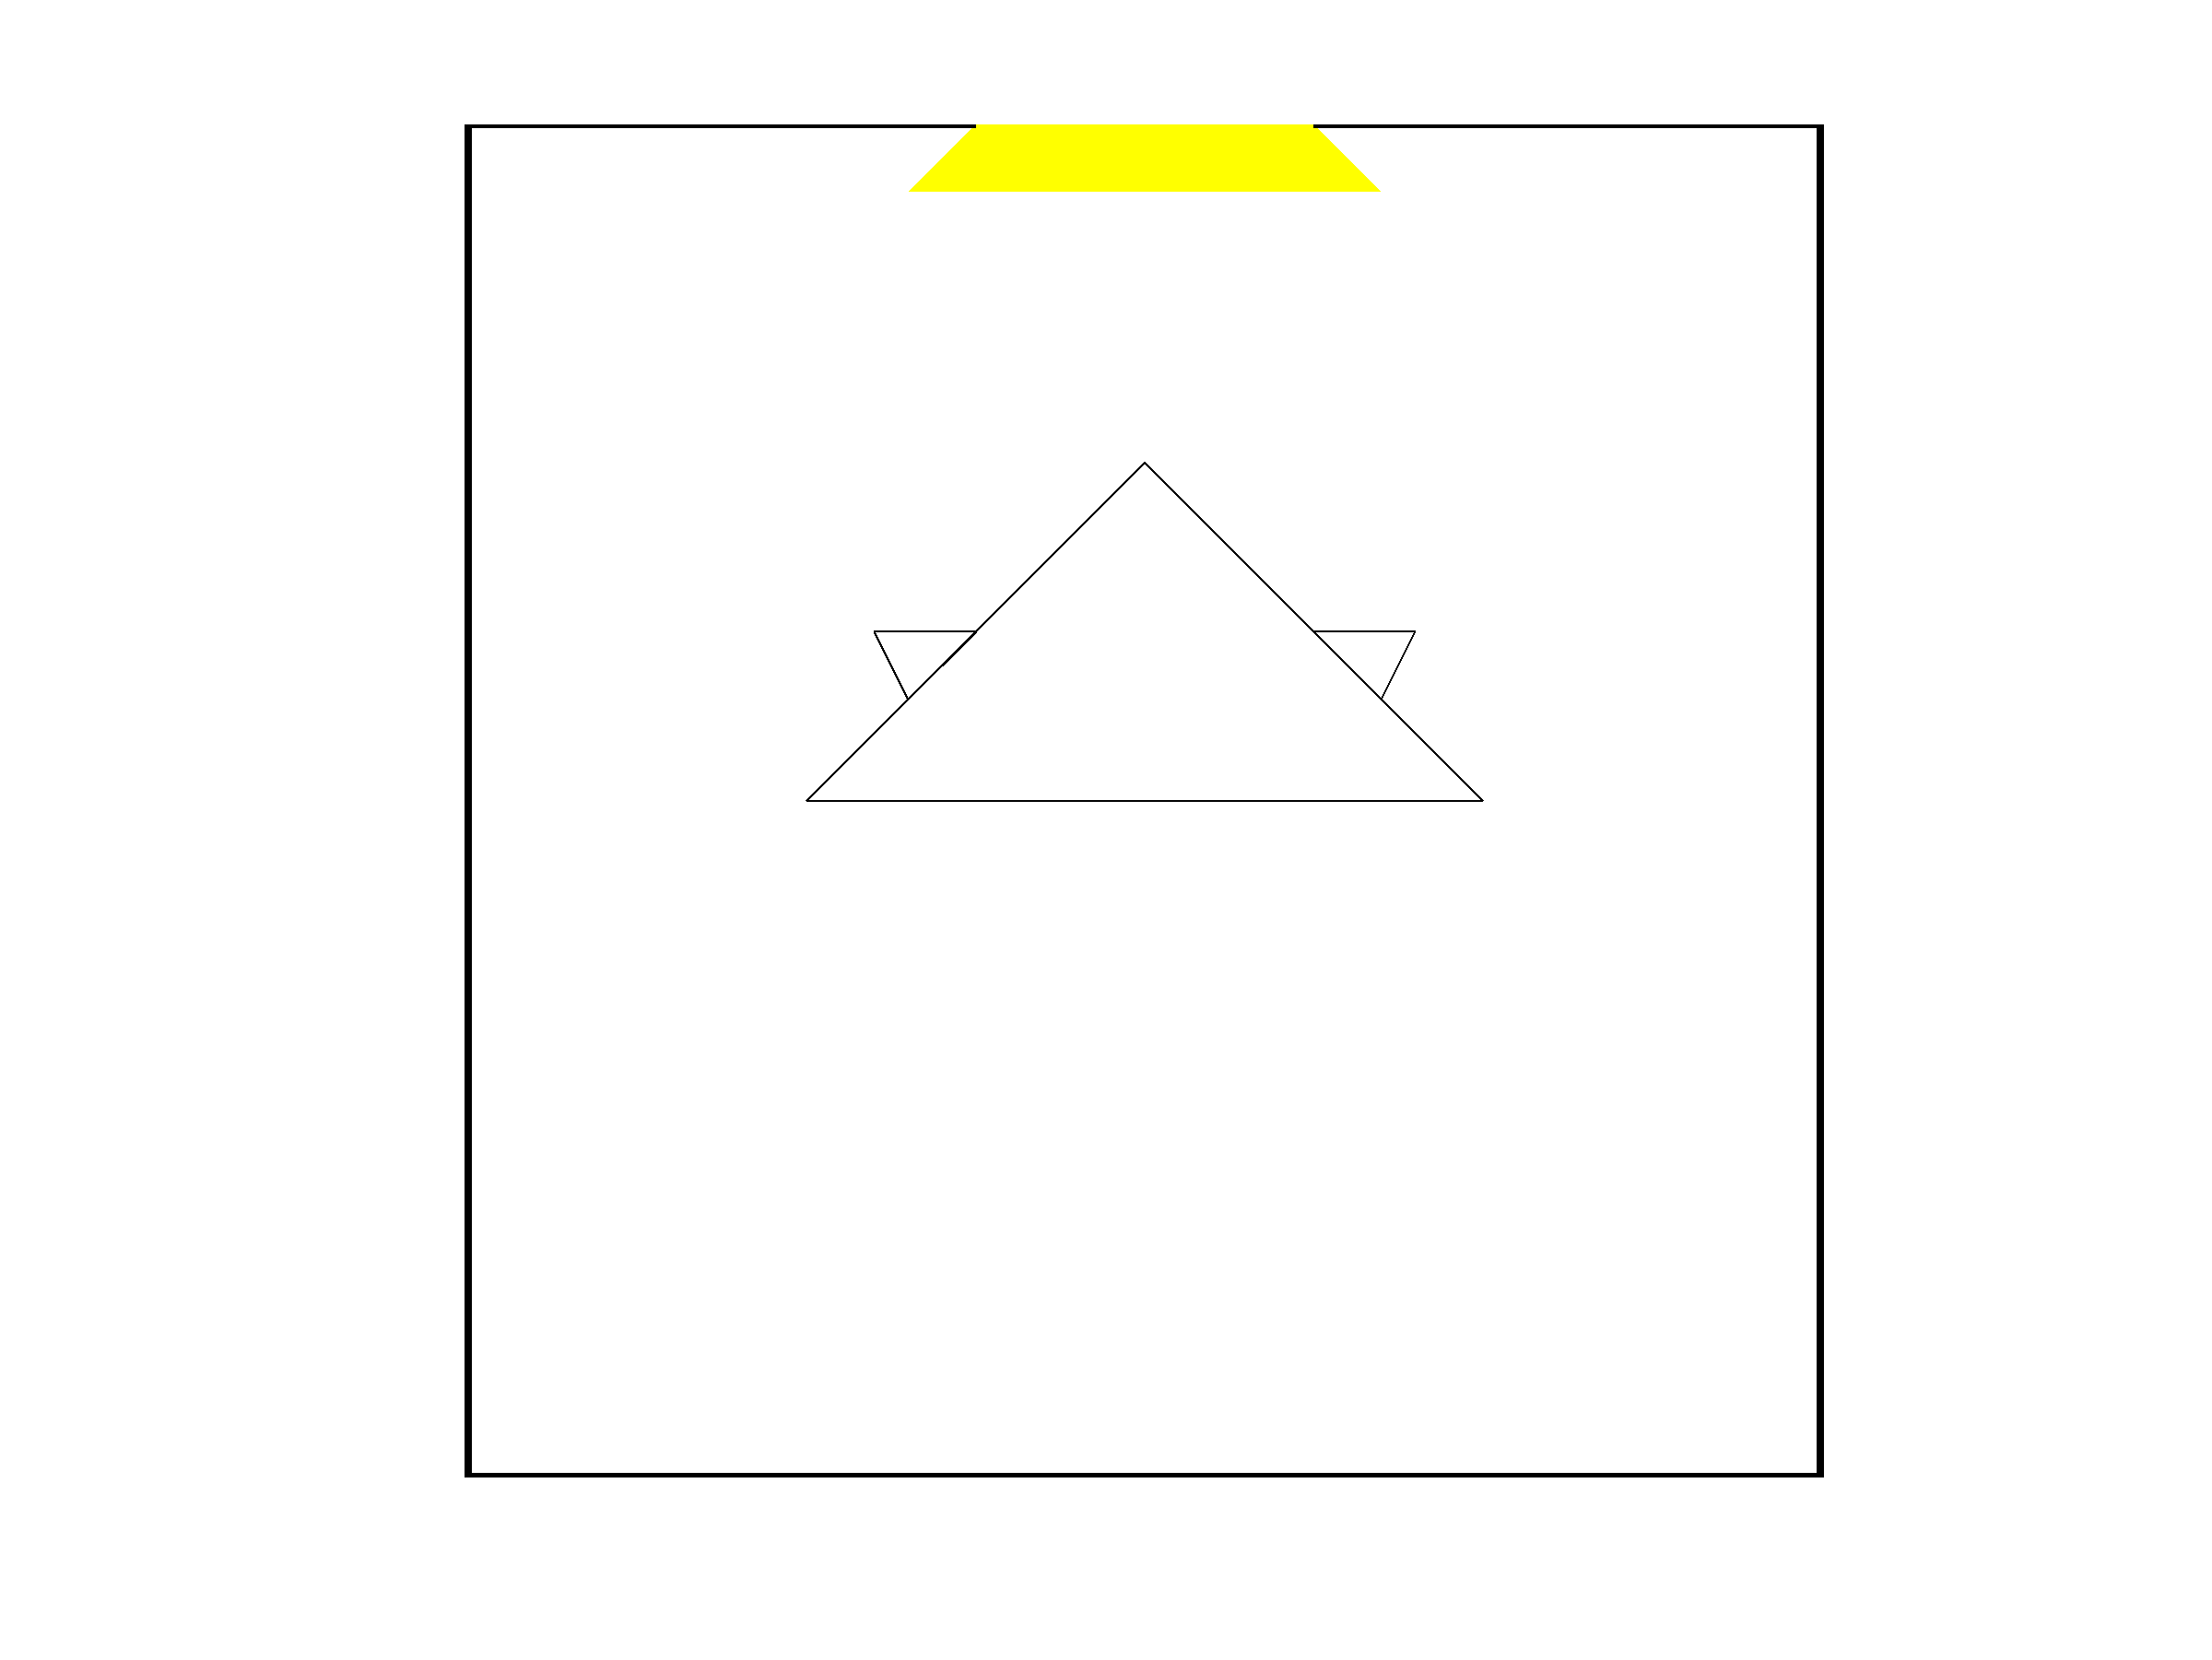
\includegraphics[width=7cm]{./fig/robot.png}
\column{6cm}
Le robot contient
\begin{itemize}
\item 2 capteurs de luminosit�s $x_1$ et $x_2$
(0 : non activ�, 1 : activ�)
\item 1 neurone (3 poids, $w_0$, $w_1$, $w_2$)
\item 1 sortie :
\begin{itemize}
\item $y=0$ : demi-tour � gauche
\item $y=1$ : avance tout droit
\end{itemize}
\end{itemize}
\end{columns}

\end{frame}
